\documentclass[a4paper]{article}

%% Language and font encodings
\usepackage[french,english]{babel}
\usepackage[utf8x]{inputenc}
\usepackage[T1]{fontenc}
\usepackage{a4wide}

%% Sets page size and margins
\usepackage[a4paper,top=3cm,bottom=2cm,left=3cm,right=3cm,marginparwidth=1.75cm]{geometry}

%% Useful packages
\usepackage{amsmath}
\usepackage{graphicx}
\usepackage[colorinlistoftodos]{todonotes}
\usepackage[colorlinks=true, allcolors=blue]{hyperref}

\title{Rapport Développement Mobile}
\author{LARUE Sebastien et CLAIN Jonathan, L3 Informatique}
\date{23/04/2018}

\begin{document}
\vspace{10mm}

\maketitle
\begin{abstract}
\Large
Dans le cadre de l'UE obligatoire de développement mobiles, il est demandé de concevoir un jeu de notre choix sur la plate-forme Android et iOS. Dans ce cadre, nous avons travaillé en binôme pour réussir à coder au mieux le projet.\\
A cet effet, nous avons combiné notre temps, volonté et motivation, ainsi que nos capacités en informatique pour pouvoir réaliser au mieux ce projet qui nous tenait à cœur.\\
Nous avons dû surmonter et pallier avec nos erreurs et faiblesses pour concevoir et répondre aux cahier des charges ainsi que pour offrir aux utilisateurs le jeu le plus attractifs et distrayants possible.\\
A la fin de trois semaines de travail, nous avons donc réussi à mettre en place ce projet, peut-être incomplet mais fonctionnel, remplissant les demandes les plus basiques de notre jeu.\\
De par sa simplicité, Smasher nous a conquis, nous concepteurs et nous espérons qu'il en sera de même pour vous, joueurs.\\
\end{abstract}

\newpage
\part*{Introduction}
\Large
Le jeu Smasher, en accord avec les cahiers des charges a donc été réalisé sur Android et sur iOS, deux conceptions complètements différentes et qui ont nécessité un éventail de compétences conséquent.\\
Ce jeu est un casse-brique datant de 1976 et dont la popularité a continué à augmenter à travers les âges. De part son côté vintage, il reste très apprécié et est un incontournable du jeu vidéo toujours aujourd'hui.\\
Nous attellerons donc à vous présenter les différentes ficelles de sa conceptions que ce soit, d'abord, à travers la version Android puis, dans un second temps, celle d'iOS.\\
Afin de réaliser ce projet, différents sites et forums nous ont été utiles tels que: \cite{AndroidStudio}, \cite{Apple} et \cite{OpenClassroom}

\section{Description}
Ce jeu reprend l’idée simple et efficace du casse brique et consiste, comme son nom l'indique, à se débarrasser des différentes briques présentent à l'aide d'une petite balle. La trajectoire de cette dernière peut être orientée grâce au paddle. Il forme également une limite pour la balle, en dessous de la quelle la balle est perdue.\\
La partie s'arrête soit lorsque que toutes les briques ont été détruites, résultant à une victoire. Ou, dès que la balle descend en dessous de la limite, équivalant à une défaite.\\
Bien que le fonctionnement soit le même, les deux versions - Android et iOS - diffèrent. Nos connaissances nous ont permis de développer et d'approfondir davantage la version Android, bien que l'esthétisme puisse être à déplorer. 
A contrario, la version iOS, bien que fonctionnelle, est plus restreinte mais aussi, plus attractive visuellement parlant.\\
La version Android se compose de cinq niveaux à la difficulté croissante qui doivent tous être réussis afin d'accéder à la victoire. Pour ce faire, le jouer ne dispose que d'une vie et, doit faire face, à chaque étapes, à de nouvelles difficultés qui sont l'augmentation de la vitesse de la balle et l'ajout d'une nouvelle ligne de huit briques.\\
La version iOS quant à elle est simplifiée. Le jeu se compose cette fois de trois lignes de quatre briques qui doivent toutes être détruite pour assurer la victoire. Le joueur ne possède encore qu'une seule vie, mais cette fois, le niveau de difficulté ne change pas.\\

\newpage
\section{Architecture générale}
\subsection{Android}
%Completer par JClain
Cette partie du rapport du rapport sera consacrée a présenter l'architecture générale de la version Android de notre projet.\\
Le projet a été réalisé sur Android Studio en langage Java.

\subsubsection{Les objets du jeu }
Le jeu est constitué de trois classes  objet qui sont les suivant:
\begin{itemize}
 \item Ball.java
 \item Brick.java
 \item Plateform.java
\end{itemize}
Ces trois classes fonctionnement en effet de la même manière. Elles possèdent toutes un constructeur permettant leur initialisation dans le jeu. C'est dans dans ces classe que l'on définie toute les caractéristiques des objets, comme par exemple la vitesse de la balle, la taille des briques ou leurs positions initiales.

\subsubsection{MainActivity.java}
C'est dans cette classe qu'on met en place le menu de notre jeu. En effet le menu se compose de deux boutons respectivement "play" et "score" mise en place dans notre premier fichier "activityMain.xml". Ainsi, c'est dans cette classe que l'on gère les événements sur les boutons et donc le lancement du jeu ou la visualisation des scores (voir partie 3.1).

\subsubsection{GameActivity.java}
C'est dans cette classe qu'on gère l'activité de notre jeu tel que le lancement du jeu et l’arrêt du jeu.\\
Elle est composée principalement de deux méthodes. Premièrement, nous avons la méthode onResume() qui va tout simplement lancer le jeu. Ensuite nous avons onPause() elle permet l’arrêt du jeu. 

\subsubsection{GameView.java}
C'est la classe principale de notre jeu. En effet c'est ici que l'on va créer les éléments du jeu. Nous avons l'initialisation de la balle, des briques et de la plate-forme. Comme les briques se génèrent en fonction des niveaux atteint par le joueur, la fonction "createBrick" est donc très utile. La méthode "Draw" permet ainsi de dessiner nos objet sur une surface définie. En effet on a utilisé Canvas, qui nous a permis de dessiner les figures.\\
Une méthode importante de cette classe est la méthode Run, qui comme son nom l'indique permet de faire tourner le jeu. C'est cette dernière fait appel aux autres méthodes du jeu dont la collision de la balle avec les murs, les briques  et la plate-forme qui sont assuré par la méthode update. Cette dernière doit s’exécuté tant que le jeu est en cours. 

\subsubsection{Score}
Au lancement du Jeu, le joueur doit renseigner son pseudo pour la partie en cours. Le score sera associé au pseudo.
\begin{center}
  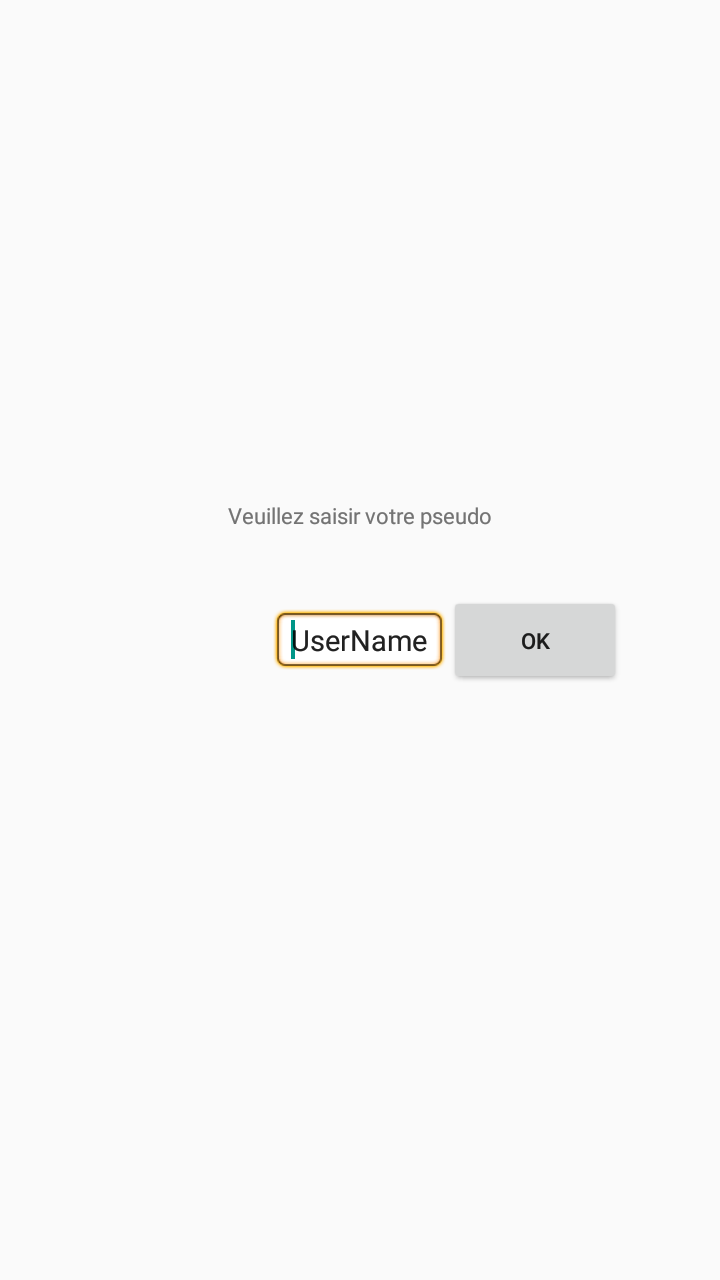
\includegraphics[scale=0.20]{images/score.png}
\end{center}
Une fois le pseudo tapé et validé, le jeu se lance.

\subsubsection{Affichage du Score}
L'affichage du score se fait sous forme de listeView. Il est donc nécessaire de créer une adaptateur d'où la classe "MyArrayAdaptater.java" qui va permettre la récupération du pseudo et du score et l'afficher dans la vue correspondante. Ainsi une autre classe appelée "Score.java" permet de mettre en place l'adaptateur.

\newpage
\subsection{iOS}
Cette partie-ci est destinée à la présentation de l'architecture générale de la version iOS de notre projet.\\
Le Casse-Brique a été réalisé sur Xcode en langage Swift avec SpriteKit.

\subsubsection{GameScene.swift}
Ce fichier coordonne l'ensemble des actions de notre jeu. On y retrouve le code qui génère les briques, affiche le score, positionne et détecte les mouvements du paddle, etc..\\
Ci-dessous est présenté le code qui ajoute de la physique en créant une barrière invisible autour de l’écran, limitant les déplacement de la balle:
\begin{verbatim}
let border = SKPhysicsBody(edgeLoopFrom: self.frame)
        border.friction = 0
        border.restitution = 1
        self.physicsBody = border
\end{verbatim}

\subsubsection{GameScene.sks}
Le fichier .sks est un éditeur de scène. Grâce a SpriteKit nous pouvons facilement générer les sprites de la balle et du paddle. Nous pouvons également changer les attributs de chacun d'entre eux présent dans le jeu. 

\subsubsection{Les 3 états}
Le jeu est constitué de trois états ("game states" en anglais) qui sont les suivant:
\begin{itemize}
 \item Tap.swift
 \item Play.swift
 \item GameOver.swift
\end{itemize}
Le premier état dans lequel se trouve notre jeu est: Tap. A ce moment, le jeu est chargé et attend que l'utilisateur tape l’écran pour débuter une partie.\\
Lorsqu'il est démarré, le jeu est en état: Play. En fonction des performances du joueur, il lui est possible de remporter la partie en détruisant toutes la briques. Dans le cas contraire, le joueur perd la balle - qui se retrouve hors des limites prévues à cet effet - et la partie se solde par un échec. Le casse-brique se retrouve ainsi en état: GameOver.
Le code qui déclare les états est le suivant:
\begin{verbatim}
lazy var gameState: GKStateMachine = GKStateMachine(states: [
        Tap(scene: self),
        Play(scene: self),
        GameOver(scene: self)])
\end{verbatim}

\section{Android: Interfaces}
Cette partie du rapport est consacrée aux divers interfaces de notre projet.\\
Le projet Android se compose:
\begin{itemize}
 \item Un menu de jeu
 \item L'interface de score
 \item L'interface de jeu
\end{itemize}

\subsection{Menu du jeu}
Sur le menu de jeu, le joueur a la possibilité de démarrer une nouvelle partie ou de regarder son score.
\begin{center}
  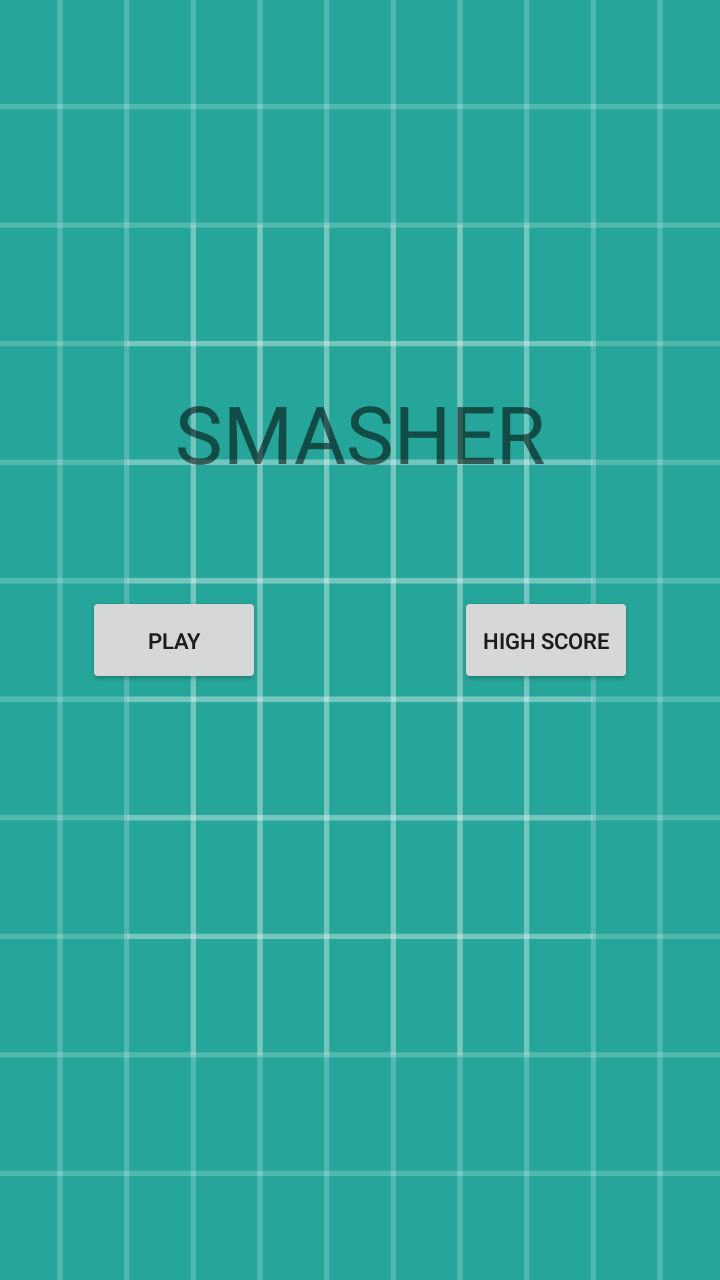
\includegraphics[scale=0.20]{images/1.png}
\end{center}

\newpage
\subsection{L'interface de score}
Par le biais de cette interface-ci, le joueur peut regarder son score.
\begin{center}
  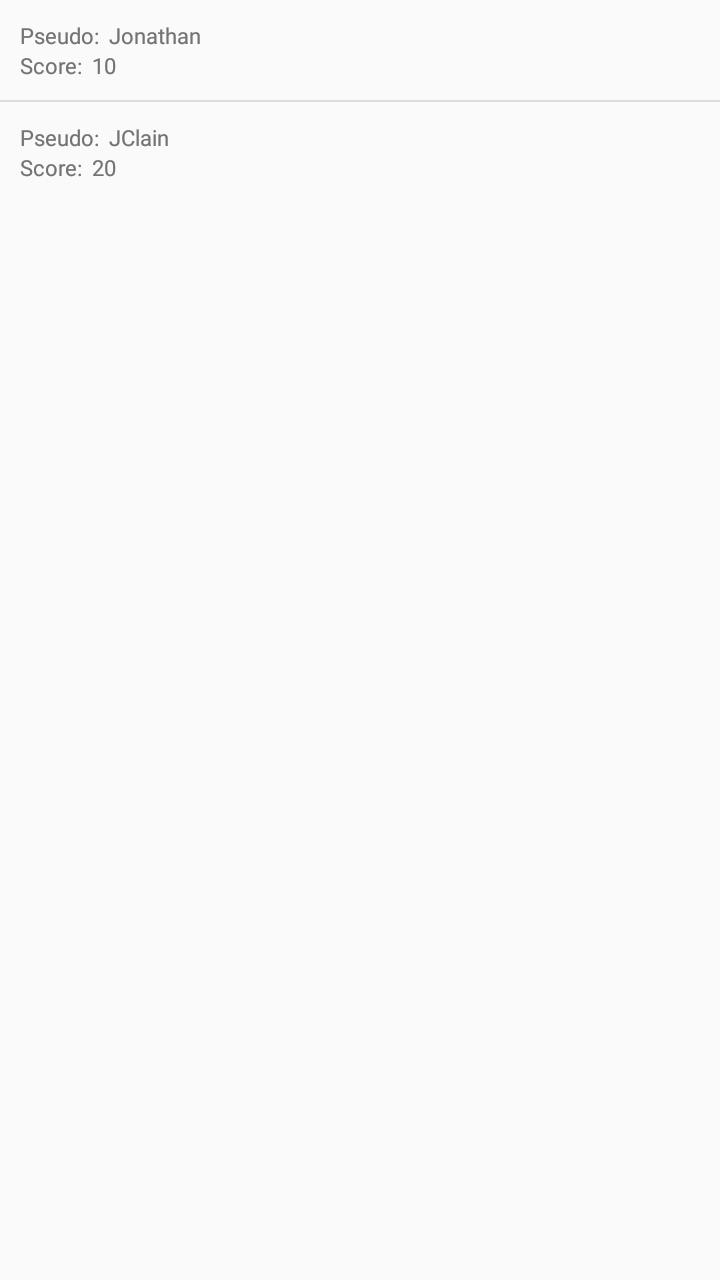
\includegraphics[scale=0.20]{images/2.png}
\end{center}

\subsection{L'interface de jeu}
Le joueur à la possibilité de démarrer une nouvelle partie en appuyant tout simplement sur l'écran.
\begin{center}
  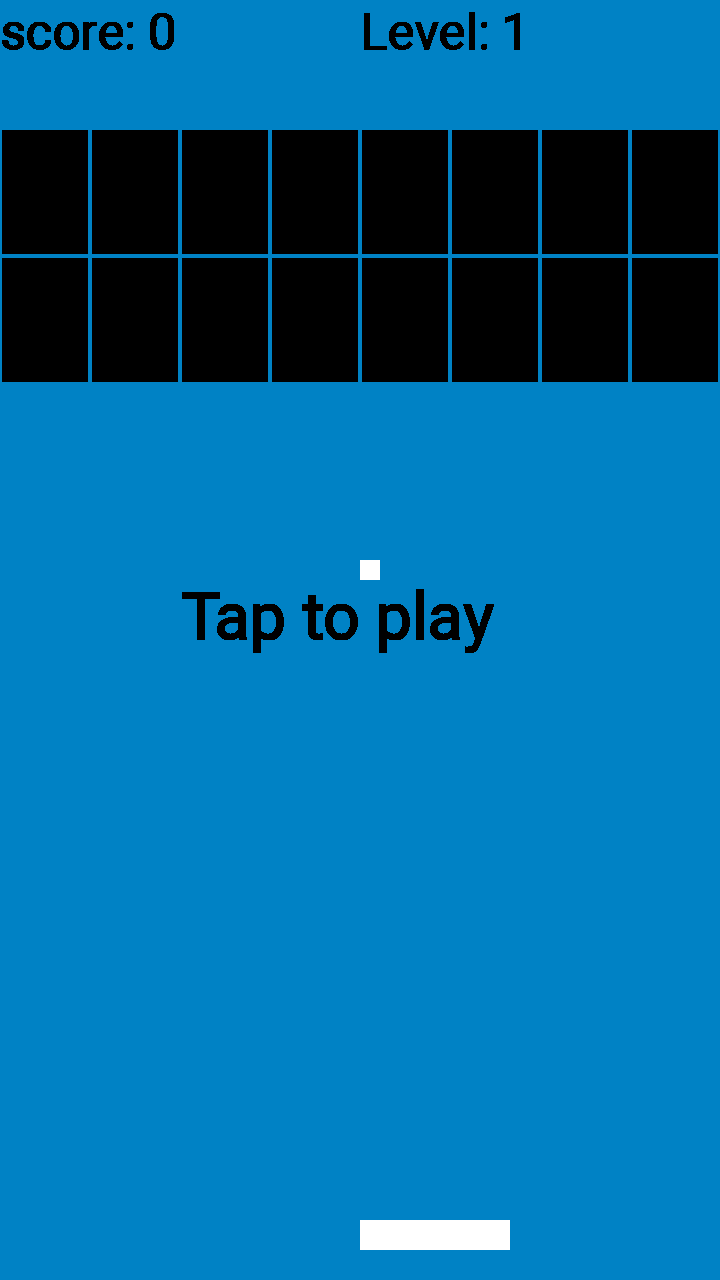
\includegraphics[scale=0.20]{images/3.png}
\end{center}

\newpage
\section{iOS: Interfaces}
\subsection{L'interface de jeu}
Comme sur la version Android, le joueur peut commencer une nouvelle partie dès lors qu'il appui sur l'écran.
\begin{center}
  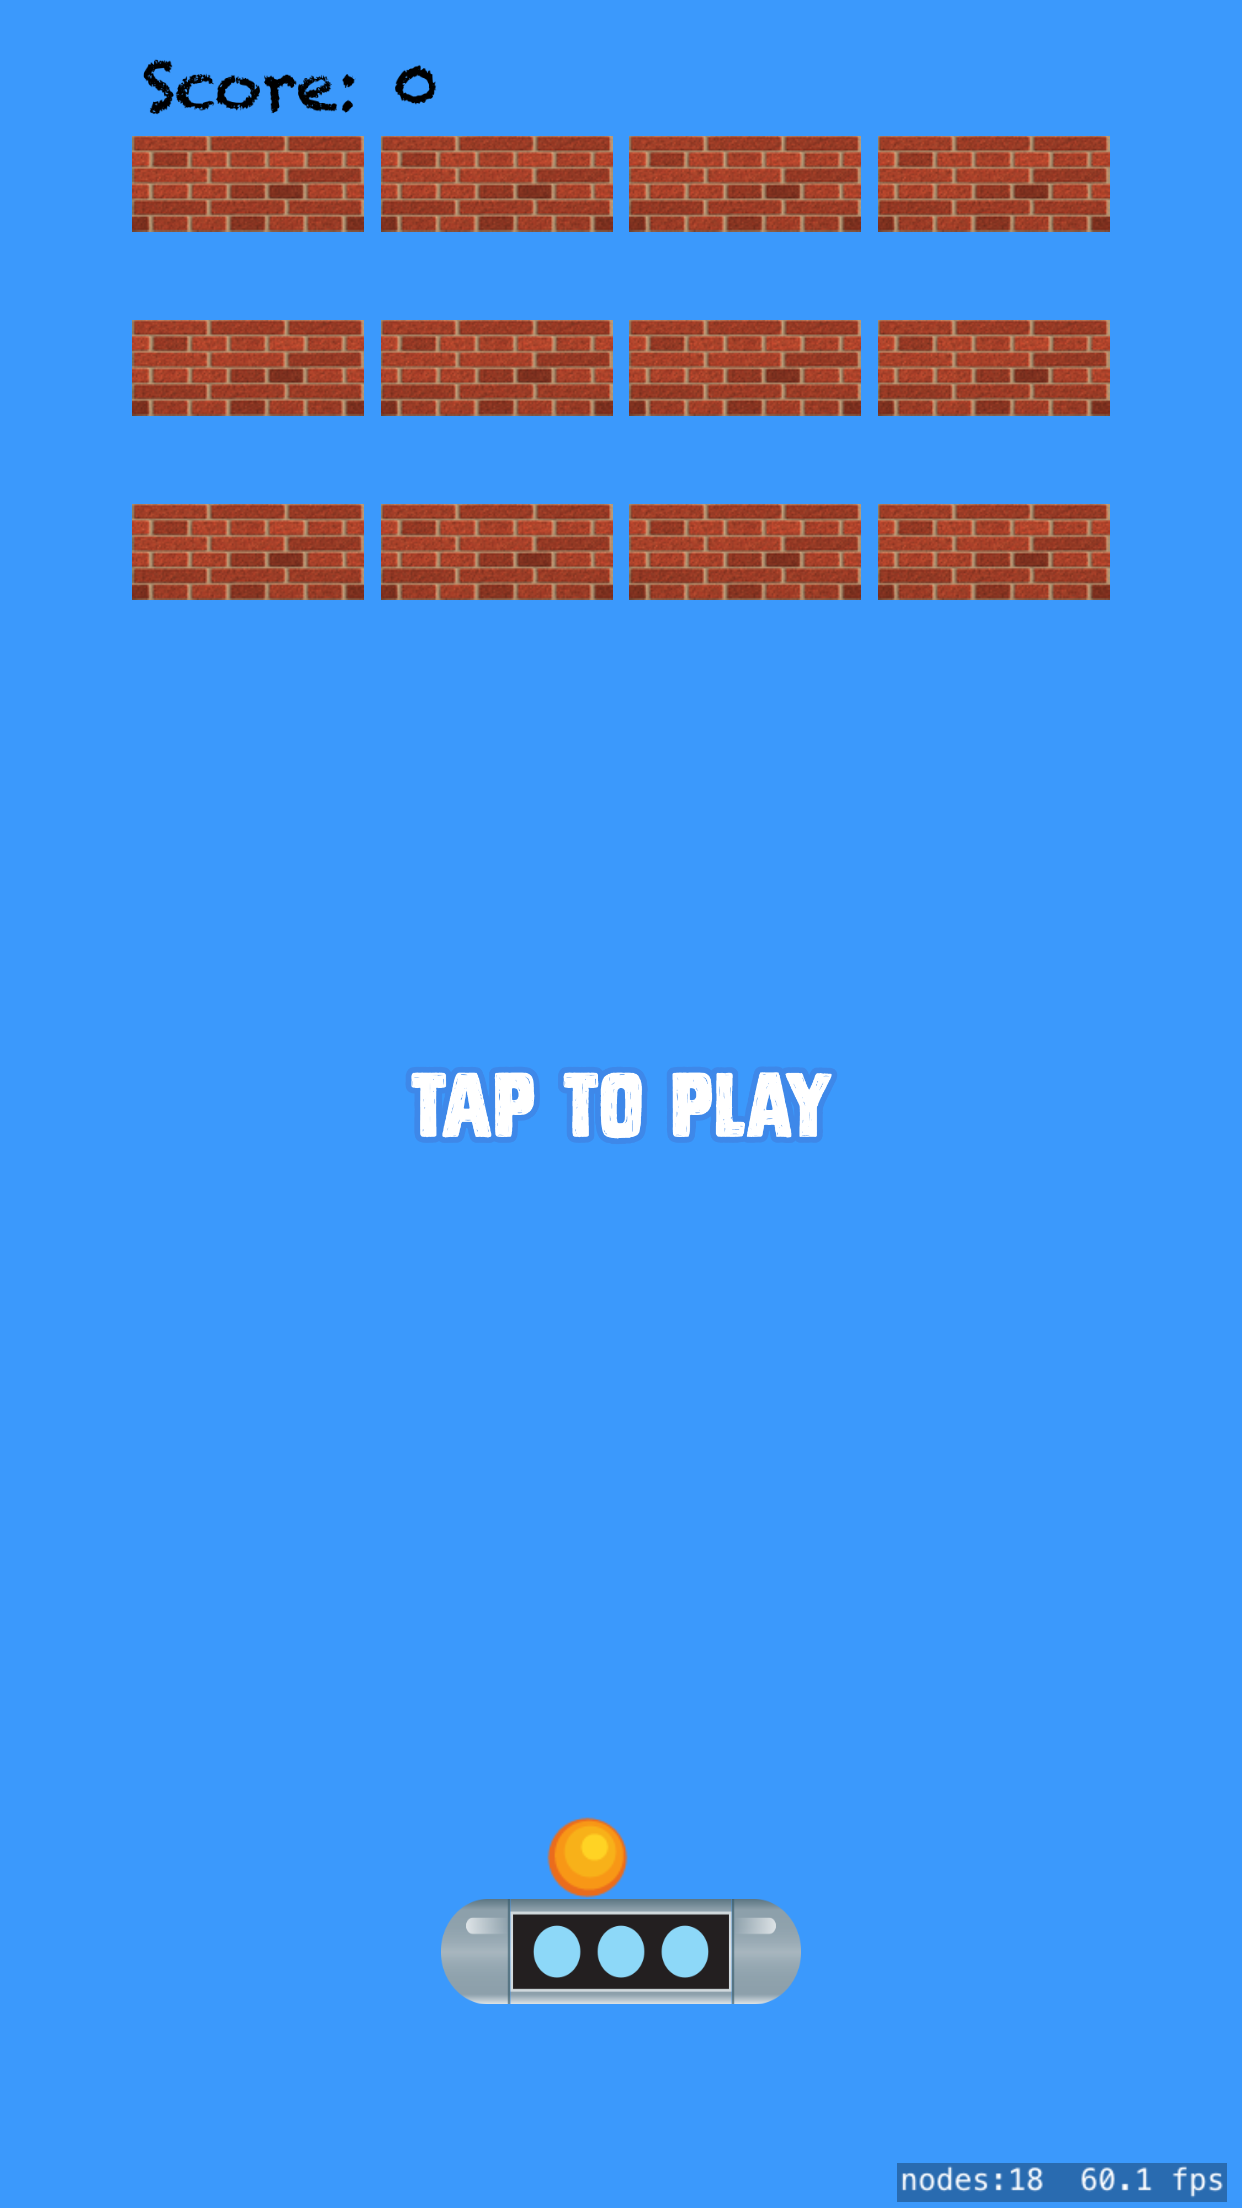
\includegraphics[scale=0.11]{images/iOS1.png}
\end{center}

\subsection{Défaite du joueur}
Quand la balle descend au-delà de la limite, le joueur perd et peut ou non, recommencer une partie
\begin{center}
  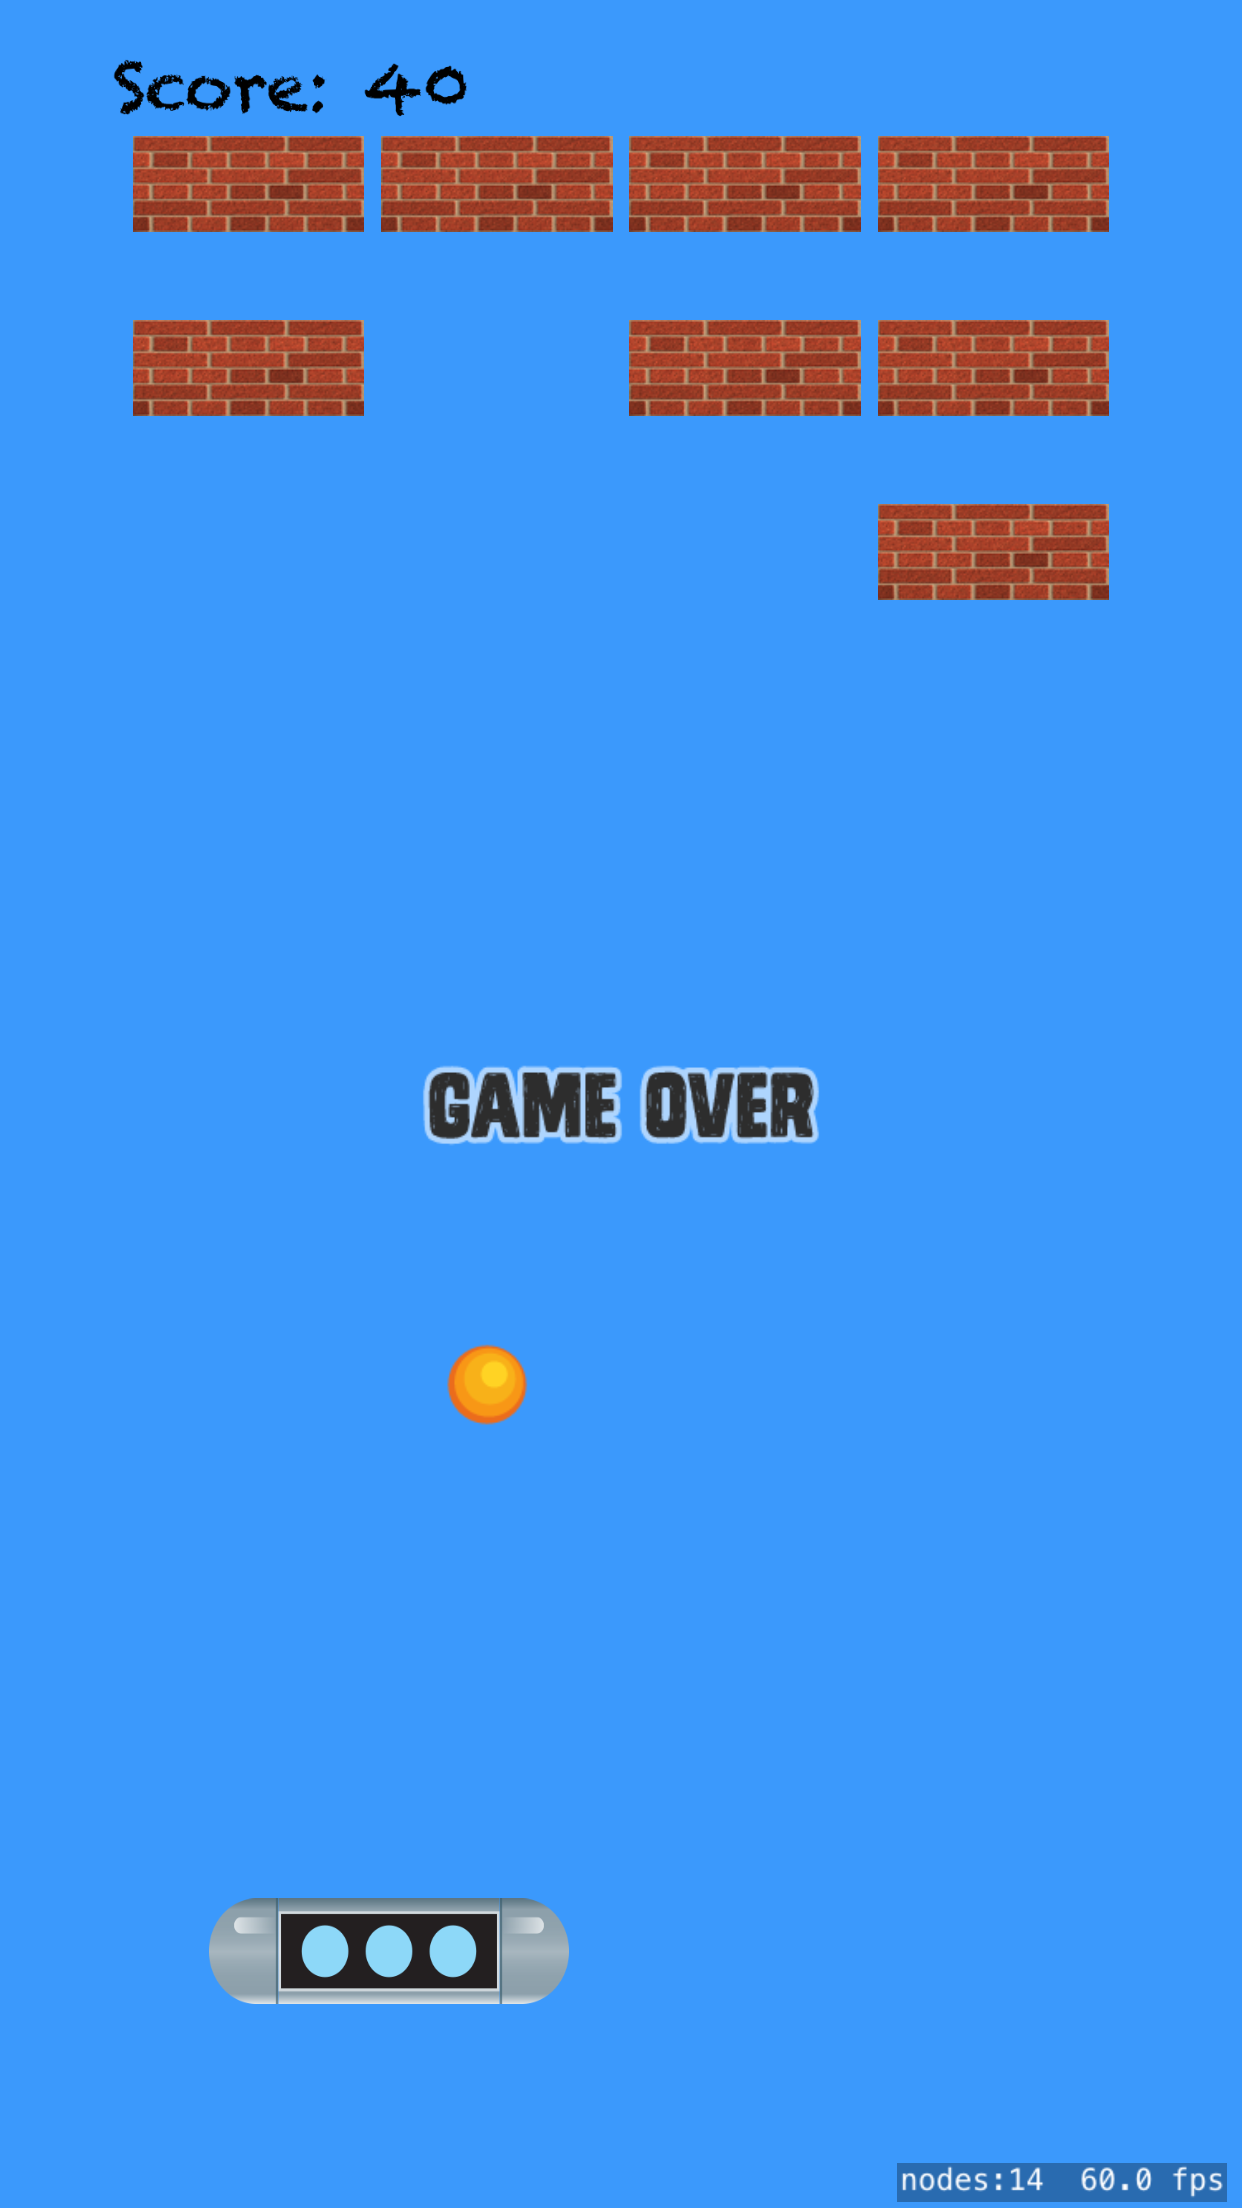
\includegraphics[scale=0.11]{images/iOS3.png}
\end{center}

\newpage
\subsection{Victoire du joueur}
Dès lors que toutes les briques ont disparu, l'objectif est rempli et la partie se solde par la victoire du joueur.
\begin{center}
  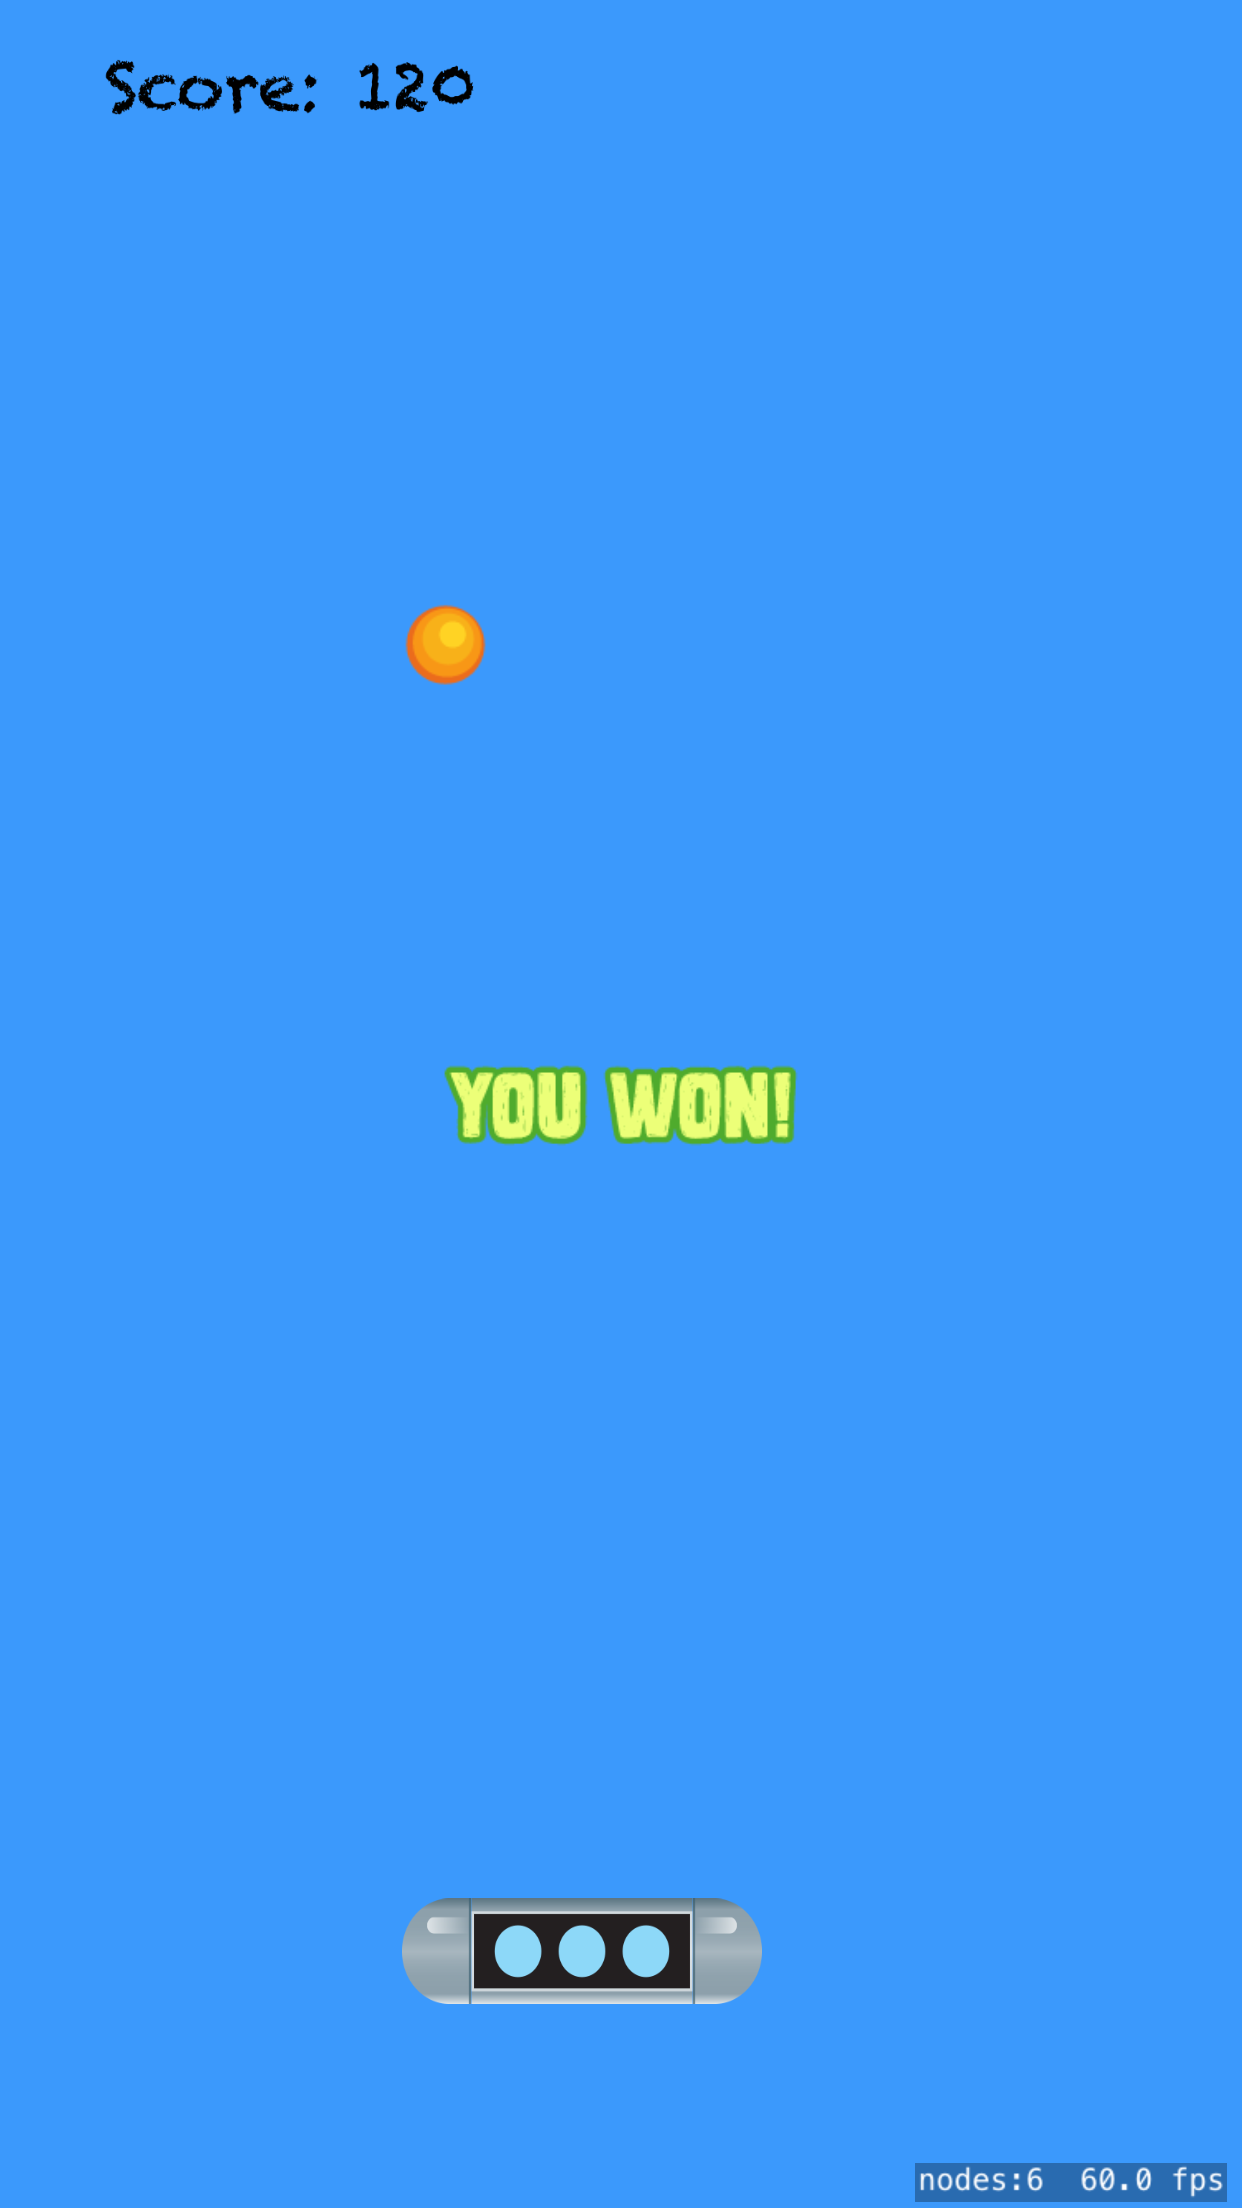
\includegraphics[scale=0.11]{images/iOS4.png}
\end{center}

\part*{Conclusion}
\Large
En conclusion, ce projet fut une belle épreuve et qui nous a permis d’acquérir de l’expérience dans le développement d'applications pour mobiles.\\
Nous en tirons énormément de points positifs.\\
Tout d'abord, ce projet nous a permis de découvrir de nouveaux outils de travail tel que Android Studio, Xcode et Beamer.Ce travail représentait un véritable défi, notamment pour la réalisation du jeu sur iOS, partie bien plus complexe autant du point de vue technique que concernant l'organisation même du travail. Nous avons du nous rendre au PTU, tous les après-midi afin d'exploiter le matériel nécessaire.Qui plus est, l'écriture de ce rapport nous a permis de de développer nos capacités rédactionnelles et d'apprendre à tirer le meilleur de ce travail afin de vous le présenter le mieux possible.\\
Sur le plan personnel, il a été très fructueux de travailler en équipe. Nous avons pu créer une véritable cohésion et mettre en place un dialogue. Ce projet nous a permis de confronter nos idées, développer notre esprit d'équipe et de mettre de côté nos différents et idées antagonistes afin de pouvoir créer le meilleur jeu possible.\\

\bibliographystyle{plain}
\bibliography{bibli}

\end{document}